%----------------------------------------------------------------------------------------
%	PACKAGES AND OTHER DOCUMENT CONFIGURATIONS
%----------------------------------------------------------------------------------------
\documentclass[paper=a4, fontsize=11pt]{scrartcl} % A4 paper and 11pt font size

\usepackage[T1]{fontenc} % Use 8-bit encoding that has 256 glyphs
\usepackage{fourier} % Use the Adobe Utopia font for the document - comment this line to return to the LaTeX default
\usepackage[english]{babel} % English language/hyphenation
\usepackage{amsmath,amsfonts,amsthm,amssymb} % Math packages
\usepackage{mathrsfs}
\usepackage{algorithm, algorithmic}
\renewcommand{\algorithmicrequire}{\textbf{Input:}} %Use Input in the format of Algorithm  
\renewcommand{\algorithmicensure}{\textbf{Output:}} %UseOutput in the format of Algorithm  
\usepackage{listings}
\lstset{language=Matlab}
\usepackage{enumerate}
\usepackage{graphicx}

\usepackage{lipsum} % Used for inserting dummy 'Lorem ipsum' text into the template
\usepackage{sectsty} % Allows customizing section commands
\allsectionsfont{\centering \normalfont\scshape} % Make all sections centered, the default font and small caps
\usepackage{fancyhdr} % Custom headers and footers
\pagestyle{fancyplain} % Makes all pages in the document conform to the custom headers and footers
\fancyhead{} % No page header - if you want one, create it in the same way as the footers below
\fancyfoot[L]{} % Empty left footer
\fancyfoot[C]{} % Empty center footer
\fancyfoot[R]{\thepage} % Page numbering for right footer
\renewcommand{\headrulewidth}{0pt} % Remove header underlines
\renewcommand{\footrulewidth}{0pt} % Remove footer underlines
\setlength{\headheight}{13.6pt} % Customize the height of the header

\numberwithin{equation}{section} % Number equations within sections (i.e. 1.1, 1.2, 2.1, 2.2 instead of 1, 2, 3, 4)
\numberwithin{figure}{section} % Number figures within sections (i.e. 1.1, 1.2, 2.1, 2.2 instead of 1, 2, 3, 4)
\numberwithin{table}{section} % Number tables within sections (i.e. 1.1, 1.2, 2.1, 2.2 instead of 1, 2, 3, 4)

\setlength\parindent{0pt} % Removes all indentation from paragraphs - comment this line for an assignment with lots of text

%----------------------------------------------------------------------------------------
%	TITLE SECTION
%----------------------------------------------------------------------------------------
\newcommand{\horrule}[1]{\rule{\linewidth}{#1}} % Create horizontal rule command with 1 argument of height

\title{	
\normalfont \normalsize 
\textsc{Shanghai Jiao Tong University, UM-SJTU JOINT INSTITUTE} \\ [25pt] % Your university, school and/or department name(s)
\horrule{0.5pt} \\[0.4cm] % Thin top horizontal rule
\huge Introduction to Numerical Analysis \\ HW9 \\ % The assignment title
\horrule{2pt} \\[0.5cm] % Thick bottom horizontal rule
}

\author{Yu Cang \\ 018370210001} % Your name

\date{\normalsize \today} % Today's date or a custom date

\begin{document}

\maketitle % Print the title

\section{Question 1}
	\begin{enumerate}[(a)]
		\item
			It's convex as $f''(x) = e^x > 0$.
		\item 
			Let
			\begin{equation}
				RHS \triangleq t f(x) + (1-t)f(y)
			\end{equation}
			\begin{equation}
				LHS \triangleq - f(tx+(1-t)y)
			\end{equation}
			It's concave as
			\begin{equation}
				\begin{aligned}
				  & RHS-LHS\\
						   = &[t x_1 x_2 + (1-t)y_1 y_2] -[t x_1 + (1-t)y_1][t x_2 + (1-t)y_2]\\
						   = &-t(1-t)(x_1 y_2 + x_2 y_1) < 0
				\end{aligned}
			\end{equation}
		\item 
			Convex.
			
		\item 
			Convex.
			
		\item 
			Convex.
			
		\item 
			Concave.

	\end{enumerate}

\section{Question 2}
	\begin{enumerate}[(a)]
		\item 
			\begin{proof}
				Suppose $x = (x_1, x_2, ... , x_m)$, then it's left to prove that
				\begin{equation}
					\frac{\partial f}{\partial x_i} = 0
				\end{equation}
				for $i=1,2, ... , m$ at $x=x^*$.
			\end{proof}
			The partial derivative of $f$ at $x=x^*$ is defined as
			\begin{equation}
				\frac{\partial f}{\partial x_i}\Big|_{x=x^*} = 
				\lim\limits_{\Delta x_i \rightarrow 0}\frac{f(x_1, x_2, ... ,x_i^* + \Delta x_i, ... , x_m) - f(x_1, x_2, ... ,x_i^*, ... , x_m)}{\Delta x_i}
			\end{equation}
			Since $f(x^*)$ is the local minimum, $f(x_1, x_2, ... ,x_i^* + \Delta x_i, ... , x_m) \geq f(x_1, x_2, ... ,x_i^*, ... , x_m)$ however $\Delta x_i$ changes.\\
			Thus
			\begin{equation}
				\frac{f(x_1, x_2, ... ,x_i^* + \Delta x_i, ... , x_m) - f(x_1, x_2, ... ,x_i^*, ... , x_m)}{\Delta x_i} \leq 0
			\end{equation} 
			if $\Delta x_i < 0$.\\
			And
			\begin{equation}
				\frac{f(x_1, x_2, ... ,x_i^* + \Delta x_i, ... , x_m) - f(x_1, x_2, ... ,x_i^*, ... , x_m)}{\Delta x_i} \geq 0
			\end{equation}  
			if $\Delta x_i > 0$.\\
			Hence, $\frac{\partial f}{\partial x_i}\Big|_{x=x^*} = 0$ as $f$ is continuously differentiable.
			Therefore, $\triangledown f(x^*) =0$.
		\item 
			\begin{proof}
				With taylor expansion of $f(x)$ at $x=x^*$
				\begin{equation}
					\begin{aligned}
						  &f(x) - f(x^*) \geq 0 \quad \quad (\text{$f(x^*)$ is the local minimum})\\
		  \Leftrightarrow &\triangledown f(x^*) \Delta x + \frac{1}{2} \Delta \xi H(x^*) \Delta \xi ^T \geq 0\\
		  \Leftrightarrow &\frac{1}{2} \Delta \xi H(x^*) \Delta \xi ^T \geq 0 \quad \quad (\text{gradient be 0})
					\end{aligned}
				\end{equation}
				where $d(\Delta \xi, x^*) \leq d(x, x^*)$, and the gradient is $0$ as been proved above.
				Thus, $ \Delta \xi H(x^*) \Delta \xi ^T \geq 0$ for any $\Delta \xi$ within the local neighbourhood of $x=x^*$.\\
				Hence $H(x^*)$ is semi-positive finite.
				
			\end{proof}
		\item 
			\begin{proof}
				($\Leftarrow$)The global minimum must be a local minimum, and the gradient is therefore 0 as $f$ is differentiable.
				
				($\Rightarrow$)As has been proved above, $\triangledown f(x^*)=0$ indicates that $f(x^*)$ is the local minimum. It's left to prove that local minimum is also global minimum for a convex function.
				Suppose there exist $x'$ s.t. 
				\begin{equation}
					f(x') < f(x^*)
				\end{equation}
				Then, by convexity
				\begin{equation}
					f(t x' + (1-t)x^*) \leq t f(x') + (1-t) f(x^*) < \leq t f(x^*) + (1-t) f(x^*) = f(x^*)
				\end{equation}
				When $t\rightarrow1$, the inequality above contradicts local optimality of $x^*$.\\
				Thus, the assumption fails, which indicates that $f(x^*)$ is the global minimum for $f$.
				
			\end{proof}
		\item
			\begin{proof}
				($\Rightarrow$)By Taylor expansion
				\begin{equation}
					f(x+ d) = f(x) + \triangledown f(x) d + \frac{1}{2} d^T H(x) d + O(||d||^2)
				\end{equation}
				If the Hessian matrix $H$ is semi-definite positive, then
				\begin{equation}
					d^T H(x) d \geq 0
				\end{equation}
				Thus
				\begin{equation}
					f(x+ d) \geq f(x) + \triangledown f(x) d
				\end{equation}
				which is the so called 1-st order condition, and it implies that the function $f$ is convex.
				
				($\Leftarrow$)By Taylor expansion
				\begin{equation}
					f(x+ t d) = f(x) + t \triangledown f(x) d + \frac{t^2}{2} d^T H(x) d + O(||d||^2)
				\end{equation}
				With the 1-st order condition
				\begin{equation}
					f(x+ t d) \geq f(x) + t \triangledown f(x) d
				\end{equation}
				Thus
				\begin{equation}
					\frac{t^2}{2} d^T H(x) d + O(t||d||^2) \geq 0
				\end{equation}
				Dividing it by $\frac{t^2}{2}$ and set $t \rightarrow 0$, it gives out that for any $d\in \mathbb{R}^n$, $d^T H(x) d \geq 0$.
				
			\end{proof}
		
	\end{enumerate}

\section{Question 4}
	The genetic algorithm is adopted as there exists intensive oscillation when $x$ approaches $0$, and optimization algorithms dependent on the gradient info are easy to fall into local minimum.\\
	The global minimum found is $x_0=0.217, f(x_0)=-0.0249$.
	
\section{Question 6}
	The plot of $g(y)$ is given as follows
	\begin{figure}[!htbp]
		\centering
		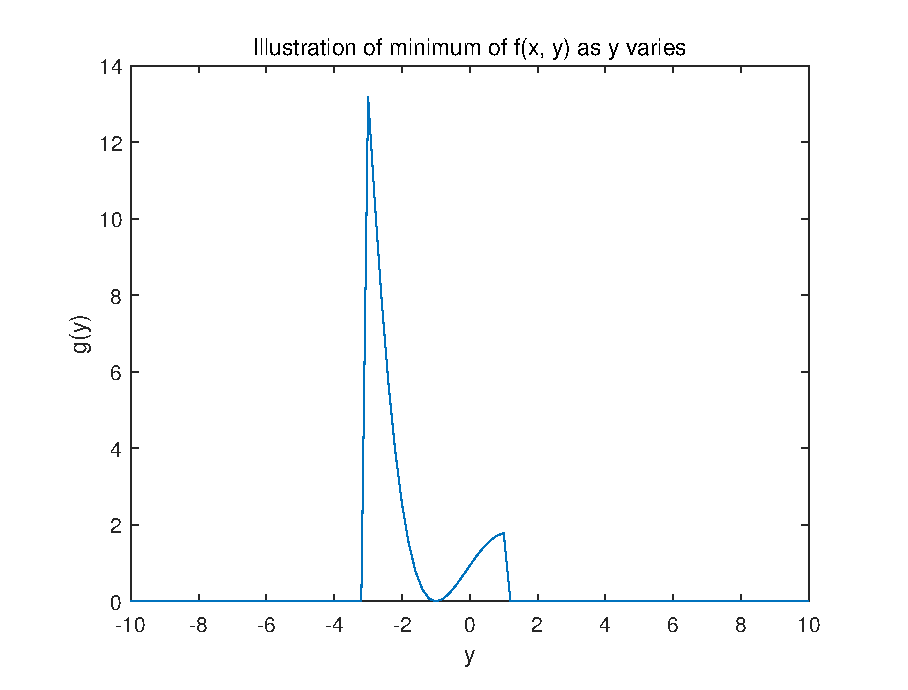
\includegraphics[width=15cm]{../pic/Task6.eps}
	\end{figure}

\section{Question 7}
	According to the geometric relations, the allowable length of the ladder is given as
	\begin{equation}
		L(\alpha) = \min\limits_{\beta} (\frac{1}{sin(\beta)} + \frac{1}{sin(\alpha + \beta)})
	\end{equation}
	By solving the minimisation problem, the plot of $L$ versus $\alpha$ is given as follows
	\begin{figure}[!htbp]
		\centering
		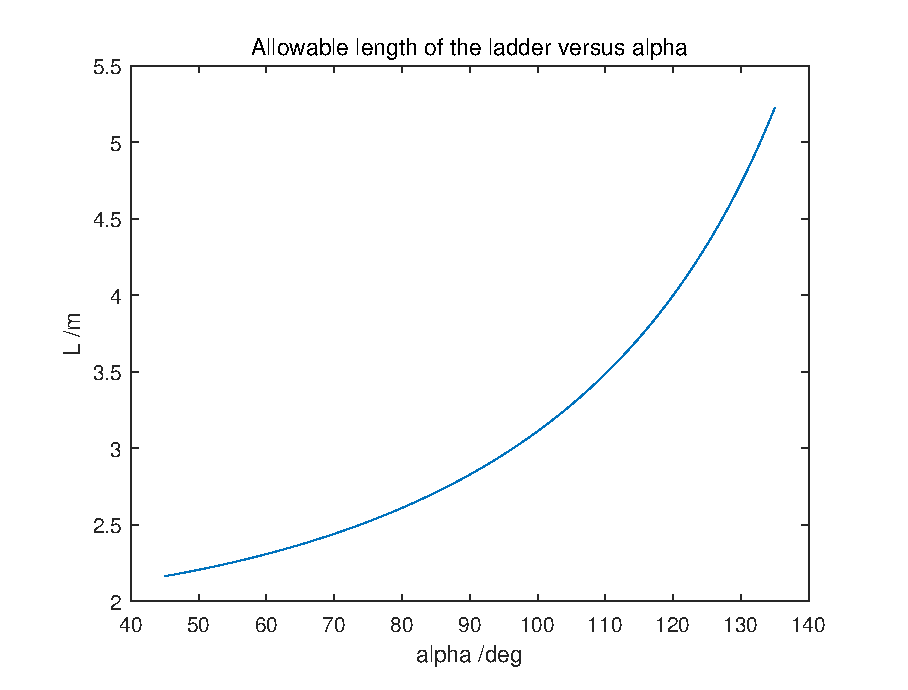
\includegraphics[width=15cm]{../pic/Task7.eps}	
	\end{figure}


\end{document}